\documentclass[10pt,a4paper]{article}
\usepackage[utf8]{inputenc}
\usepackage[english]{babel}
\usepackage{csquotes}
\usepackage{amsmath}
\usepackage{amsfonts}
\usepackage{amssymb}
\usepackage{graphicx}
\usepackage[margin=0.5in]{geometry}
\usepackage{amsthm}
\usepackage{enumitem}
\usepackage{tikz}
\usetikzlibrary{calc}
\newtheorem{question}{Question}
\newtheorem*{question*}{Question}
\newtheorem{theorem}{Theorem}
\newtheorem*{theorem*}{Theorem}
\newtheorem{lemma}{Lemma}

\theoremstyle{definition}
\newtheorem{answer}{Answer}
\newtheorem*{answer*}{Answer}

\theoremstyle{definition}
\newtheorem{verify}{Verification}
\newtheorem*{verify*}{Verification}

\numberwithin{equation}{section}


\title{Applied Math HW 4}
\author{Colin Williams}

\begin{document}
\maketitle

\section*{Question 1}
Let $u$ and $v$ be vectors in $\mathbb{R}^n$, and let $A$ and $B$ be two $n \times n$ matrices. 
\begin{enumerate}[label = (\alph*)]
\item Find the number of operations (multiplications and divisions) required to compute the scalar product, the norm $||u||_2$ and the rank-one matrix $uv^T$. 
	\begin{itemize}
	\item Let $u = (u_1, u_2, \ldots, u_n)$ and $v = (v_1, v_2, \ldots, v_n)$. Then, the scalar product is calculated at
	\begin{align*}
	\langle u, v \rangle = u^T v = u_1v_1 + u_2 v_2 + \cdots + u_n v_n.
	\end{align*}
	Since we are only counting multiplications and divisions, we can clearly see from above that this has one multiplication for each index of the vectors, therefore \boxed{N_{op}(n) = n.}
	\item Recall that $||u||_2 = \sqrt{\langle u, u \rangle }$. We saw from before that the inner product takes $n$ multiplications to complete. If we consider the square root function as an operation, we have $N_{op}(n) = n + 1$, but if we only consider multiplications and divisions, then \boxed{N_{op}(n) = n.}
	\item Notice, the multiplication $uv^T$ is expressed as
	\begin{align*}
	uv^T = \begin{bmatrix}
	u_1\\u_2\\ \vdots \\ u_n
	\end{bmatrix} \begin{bmatrix}
	v_1 & v_2 & \cdots & v_n
	\end{bmatrix} = \begin{bmatrix}
	u_1v_1 & u_1v_2 & \cdots & u_1v_n\\
	u_2v_1 & u_2v_2 & \cdots & u_2v_n\\
	\vdots & \vdots & \ddots & \vdots\\
	u_nv_1 & u_nv_2 & \cdots & u_nv_n
	\end{bmatrix}
	\end{align*}
	Thus, notice each entry of the resulting $n \times n$ matrix has one multiplication. Therefore, there there are clearly \boxed{N_{op}(n) = n^2} operations involved. 
	\end{itemize}
\item For $n = 100k$ with $k =1, 2, \ldots, 5$, estimate the running time of Matlab (using \verb!tic! and \verb!toc!) for computing the product of two matrices $A$ = \verb!rand(n, n)! and $B$ = \verb!rand(n, n)!. Plot this running time in terms of $n$. 
	\begin{itemize}
	\item Below is my graph of the running time in terms of $n$. The size of the matrix $n$ is the horizontal axis and the running time in seconds to compute $AB$ is the vertical axis. To prevent inconsistencies from the randomness of the matrices, I did 100 matrix multiplications for each value of $n$ and averaged the computation times. I then took this average running time for a fixed $n$ to be my representative value for the plot which gave much smoother results. Additionally, I found that running my \verb!for! loop gave better results when starting at $k = 5$ and working backwards to $k = 1$ (perhaps because of MATLAB needing to load certain packages on the first use of \verb!tic! and \verb!toc!; thus, a smaller relative error when the first usage is on the longer test-case). 
	\begin{center}
	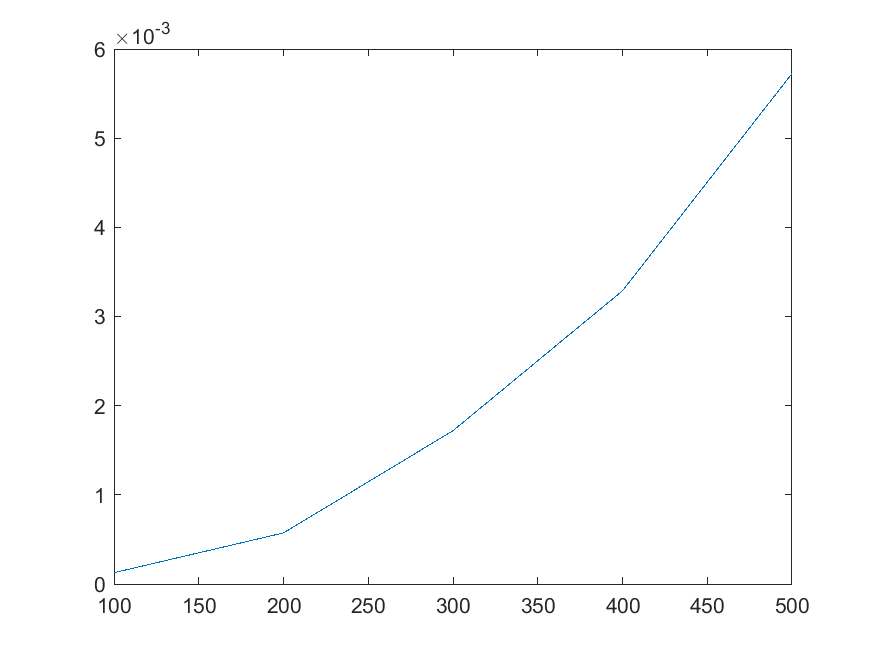
\includegraphics[scale=.8]{Time Plot}
	\end{center}
	\item The values that are represented in this graph are
	\begin{center}
	\begin{tabular}{ |c|c| } 
 	\hline
 	$n$ & time\\ 
 	\hline
 	100 & $1.2685 \times 10^{-4}$\\ 
 	200 & $5.7295 \times 10^{-4}$\\ 
 	300 & $1.7192 \times 10^{-3}$\\
 	400 & $3.2887 \times 10^{-3}$\\
 	500 & $5.7249 \times 10^{-3}$\\
 	\hline
	\end{tabular}
	\end{center}
	\item My code to produce this plot is as follows:
	\\ \begin{verbatim}
N = 100; %Number of times to average each test case
M = 5; %Max value for k
time = zeros(1, M);
n = 100*(1:M);
y = zeros(M, N);

%for k = 1:M
for k = M:-1:1
    C = zeros(n(k), n(k));
    for j = 1:N
        A = rand(n(k), n(k));
        B = rand(n(k), n(k));
        tic;
        C = A*B;
        y(k, j) = toc;
    end
    time(k) = mean(y(k, :));
end


figure;
plot(n, time);
	\end{verbatim}
	\end{itemize}
\item Assume that this running time is a polynomial of $n$, so that for $n$ large enough, $T(n) \approx Cn^s$. In order to find a numerical approximation of the exponent $s$, plot the logarithm of $T$ in terms of the logarithm of $n$. Deduce an approximate value of $s$. 
	\begin{itemize}
	\item We have seen in class that the standard algorithm for matrix multiplication takes $O(n^3)$ operations. MATLAB; however, may have a slightly more efficient algorithm, but we should expect it to be similar. Notice the following:
	\begin{align*}
	T(n) &\approx Cn^s\\
	\implies \log(T(n)) &\approx \log(Cn^s)\\
	\implies \log(T(n)) &\approx s\log(n) + \log(C)
	\end{align*}
	Therefore, when graphing the logarithm of $T$ versus the logarithm of $n$, we should expect our $s$ to be the slope of the log-log plot. With this in mind, I appended the following code to the end of the code in the previous section:
	\begin{verbatim}
figure;
w = log(n);
z = log(time);
plot(w, z)

p = polyfit(w, z, 1);
slope = p(1);
	\end{verbatim}
	\item The first 4 lines of code produced the following graph:
	\begin{center}
	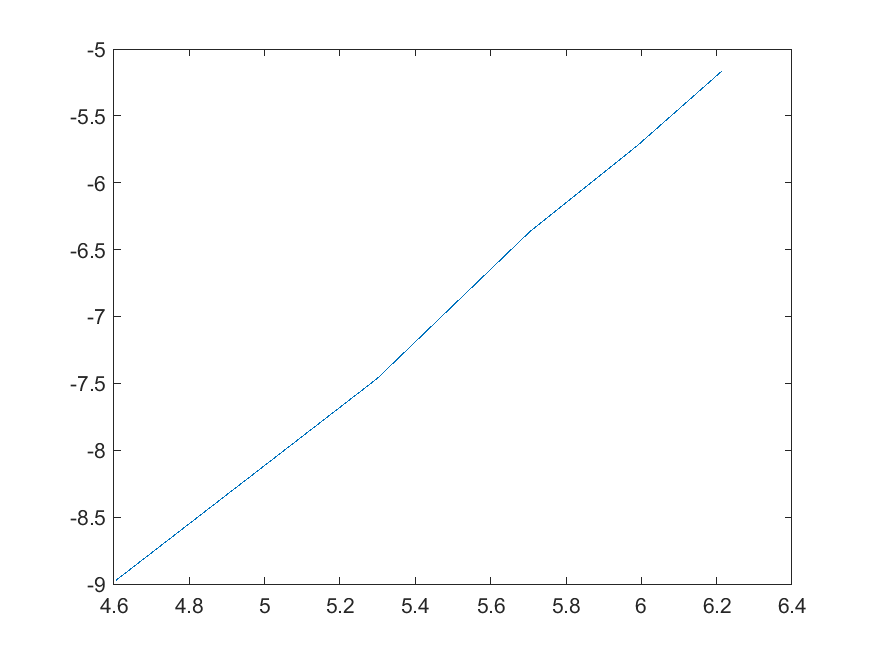
\includegraphics[scale=.8]{LogLog}
	\end{center}
	\item This graph has points at the following values:
		\begin{center}
	\begin{tabular}{ |c|c|c| } 
 	\hline
 	$n$  & $\ln(n)$ & $\ln$(time)\\ 
 	\hline
 	100 & 4.6052 & $-8.9725$\\ 
 	200 & 5.2983 & $-7.4647$\\ 
 	300 & 5.7038 & $-6.3659$\\
 	400 & 5.9915 & $-5.7173$\\
 	500 & 6.2146 & $-5.1629$\\
 	\hline
	\end{tabular}
	\end{center}
	\item The last two lines of code I added create a linear approximation of this log-log plot and then return the slope of the that line into the variable named \verb!slope!. The output of this was 2.3824 which indicates that \boxed{s \approx 2.3824}. This approximation may not be completely accurate due the randomness involved and the fact we are only using 5 test cases with a maximum $n$ of 500. More test cases and a larger set of $n$'s would likely make this estimate more accurate. 
	\end{itemize}
\end{enumerate}


\section*{Question 2}
Let $A$ be an invertible $n \times n$ matrix. Prove the following properties:
\begin{enumerate}[label = (\alph*)]
\item cond$(\alpha A) = $ cond$(A)$ for all nonzero $\alpha$. 
	\begin{itemize}
	\item Let $\alpha \neq 0$. 
	\item In order to prove the given statement, I will first prove the following property that if $A$ is invertible, then
	\begin{align*}
	(\alpha A)^{-1} = \frac{1}{\alpha} A^{-1}
	\end{align*}
	To show this, simply note that
	\begin{align*}
	(\alpha A) \left(\frac{1}{\alpha} A^{-1} \right) = \frac{\alpha}{\alpha} A A^{-1} = I\\
	\left(\frac{1}{\alpha} A^{-1} \right) (\alpha A) =\frac{\alpha}{\alpha} A^{-1}A = I
	\end{align*}
	\item Therefore, we can compute the condition number:
	\begin{align*}
	\text{cond}(\alpha A) = ||\alpha A||\;||(\alpha A)^{-1}|| = |\alpha|\; ||A||\; \left| \left| \frac{1}{\alpha} A^{-1} \right| \right| = \frac{|\alpha|}{|\alpha|} ||A|| \; ||A^{-1}|| = \text{cond}(A)
	\end{align*}
	\end{itemize}
\item cond$_2(AU) = $ cond$_2(UA) = $ cond$_2(A)$ for any orthogonal matrix $U$. 
	\begin{itemize}
	\item Recall from HW2, we have proven that $||QAZ||_2 = ||A||_2$ for $Q$ and $Z$ orthogonal matrices. In particular, by taking $Q = I$ and $Z = U$, we get $||AU||_2 = ||A||$ and by taking $Q = U$ and $Z = I$, we get $||UA||_2 = ||A||$. Note, we can also replace $A$ with $A^{-1}$ and $U$ with $U^{-1} = U^T$ (which must be also be orthogonal) and these equalities will still hold true. Therefore, we can compute the condition numbers as:
	\begin{align*}
	\text{cond}_2(AU) = ||AU||_2 ||(AU)^{-1}||_2 = ||A||_2 ||U^T A^{-1}||_2 = ||A||_2 ||A^{-1}||_2 = \text{cond}_2(A)\\
	\text{cond}_2(UA) = ||UA||_2 ||(UA)^{-1}||_2 = ||A||_2 ||A^{-1} U^T||_2 = ||A||_2 ||A^{-1}||_2 = \text{cond}_2(A)\\
	\end{align*}
	\end{itemize}
\item $n^{-2}$cond$_1(A) \leq $ cond$_\infty (A) \leq n^2$ cond$_1(A)$. 
	\begin{itemize}
	\item Recall the following property about matrix norms: $\frac{1}{n}||A||_\infty \leq ||A||_1 \leq n ||A||_\infty$. These can also be rephrased as $\frac{1}{n}||A||_1 \leq ||A||_\infty \leq n||A||_1$ which lead to:
	\begin{align*}
	\text{cond}_\infty (A) = ||A||_\infty ||A^{-1}||_\infty \leq \bigg(n||A||_1 \bigg) \bigg(n ||A^{-1}||_1 \bigg) = n^2 \text{cond}_1(A)\\
	\text{cond}_\infty (A) = ||A||_\infty ||A^{-1}||_\infty \geq \bigg(\frac{1}{n}||A||_1 \bigg) \bigg(\frac{1}{n} ||A^{-1}||_1 \bigg) = \frac{1}{n^2} \text{cond}_1(A)\\
	\end{align*}
	Putting these inequalities together clearly gives the stated property. 
	\end{itemize}
\end{enumerate}


\section*{Question 3}
Let $A$ be an invertible $n \times n$ matrix and $b$ be a nonzero vector in $\mathbb{R}^n$. Assume that $x$ and $x + \Delta x$ solve
\begin{align*}
Ax = b, && (A + \Delta A)(x + \Delta x) = b.
\end{align*}
Prove that the inequality
\begin{align*}
\frac{||\Delta x||}{||x + \Delta x||} \leq \text{cond}(A)\frac{||\Delta A||}{||A||}
\end{align*}
is optimal in the sense that there are $\Delta A \neq 0$ and $b \neq 0$ such that the equality happens. 


\begin{proof}$ $
\\We have already shown that the inequality holds in class; therefore, I simply need to show that it is an optimal inequality.
\\
\\By the definition of the operator norm, we know that there exists some vector $x_0 \neq 0 \in \mathbb{R}^n$ such that $||A^{-1}x_0|| = ||A^{-1}|| \, ||x_0||$. Define $b = x_0$. So that $Ax = b \implies x = A^{-1}b \implies ||x|| = ||A^{-1}|| \, ||b||$. With this in mind, define
\begin{align*}
\Delta A := \frac{b (x + \Delta x)^T}{||x + \Delta x||^2}
\end{align*}
With this in mind, notice the following properties:
\begin{equation}\label{Eq.b}
\Delta A(x + \Delta x) = b \frac{(x + \Delta x)^T (x + \Delta x)}{||x + \Delta x||^2} = b \frac{||x + \Delta x||^2}{||x + \Delta x||^2} = b
\end{equation}
Furthermore, we have 
\begin{align}\label{Norm.A}
||\Delta A|| = \frac{||b(x + \Delta x)^T||}{||x + \Delta x||^2} = \max_{||z|| = 1} \frac{||b(x + \Delta x)^T z||}{||x + \Delta x||^2} = \max_{||z|| = 1}\frac{|\langle x + \Delta x, z\rangle | \, ||b||}{||x + \Delta x||^2} &= \frac{||b||}{||x + \Delta x||} \nonumber\\
\implies ||\Delta A|| \, ||x + \Delta x|| &= ||b||
\end{align}
Notice the last equality in the first line of equalities above follows as an inequality with Cauchy-Schwartz and it is attained by taking $z = (x + \Delta x)/||x + \Delta x||$. Therefore, we get
\begin{align*}
(A + \Delta A)(x + \Delta x) &= b\\
\implies Ax + A \Delta x + \Delta A(x + \Delta x) &= b\\
\implies A \Delta x + \Delta A(x + \Delta x) &= 0 &\text{since $Ax = b$}\\
\implies -A^{-1} \Delta A(x + \Delta x) &= \Delta x
\end{align*}
Therefore, by taking norms of both sides of this equality, we get:
\begin{align*}
||\Delta x|| &= ||A^{-1} \Delta A (x + \Delta x)||\\
&= ||A^{-1} b|| &\text{by \eqref{Eq.b}}\\
&= ||A^{-1}||\, ||b|| &\text{by construction of $b$}\\
&= ||A^{-1}|| \, ||\Delta A|| \, ||x + \Delta x|| &\text{by \eqref{Norm.A}}\\
\implies \frac{||\Delta x||}{||x + \Delta x||} &= ||A^{-1}|| \, ||\Delta A||\\
&= ||A|| \, ||A^{-1}|| \frac{||\Delta A||}{||A||}\\
&= \text{cond}(A) \frac{||\Delta A||}{||A||}
\end{align*}
\end{proof}
Notice I was being slightly deceiving in the preceding proof by using the fact that $y^T y = \langle y, y \rangle = ||y||^2$ which is only true for the vector 2-norm. To make this proof work for the vector $p$ norm in general take
\begin{align*}
\Delta A = \frac{by^T}{||x + \Delta x||_p^2}
\end{align*}
where $y$ is chosen such that $y^T (x + \Delta x) = ||x + \Delta x||_p^2$. This $y$ will vary depending on $p$, for example
\begin{itemize}
\item $p = 1$. Take $y = ||x + \Delta x||_1 (\pm 1, \pm 1, \ldots, \pm 1)^T$ where you choose $+$ or $-$ to match the sign of $x + \Delta x$ in that coordinate. 
\item $p = \infty$. Take $y = \pm ||x + \Delta x||_\infty e_k$ where $k$ is chosen as the coordinate corresponding the largest absolute value of an entry of $x + \Delta x$ and $+$ or $-$ matches the sign of that element. 
\end{itemize}


\end{document}